%%%%%%%%%%%%%%%%%%%%%%%%%%%%%%%%%%%%%%%%%
%
% (c) 2020 by Jennifer Laaser
%
% This work is licensed under the Creative Commons Attribution-NonCommercial-ShareAlike 4.0 International License. To view a copy of this license, visit http://creativecommons.org/licenses/by-nc-sa/4.0/ or send a letter to Creative Commons, PO Box 1866, Mountain View, CA 94042, USA.
%
% The current source for these materials is accessible on Github: https://github.com/jlaaser/pogil-polymers
%
%%%%%%%%%%%%%%%%%%%%%%%%%%%%%%%%%%%%%%%%%

\renewcommand{\figpath}{content/polymchem/copolymers/copolym/figs}
\renewcommand{\labelbase}{copolym}

\begin{activity}{Copolymerization}

\begin{instructornotes}
	This activity introduces students to concepts related to the chemistry of copolymerization in chain-growth polymerizations
	
	After completing this activity, students will be able to:
	\begin{enumerate}
		\item Relate reactivity ratios to the kinetics of monomer addition in statistical copolymerizations
		\item Predict what type of polymer sequence should arise from different reactivity ratios
		\item Relate polymer compositions to feed ratios
		\item Determine the reactivity ratios from experimental data about polymer composition
	\end{enumerate}
	
	\subsection*{Activity summary:}
	\begin{itemize}
		\item \textbf{Activity type:} Learning Cycle
		\item \textbf{Content goals:} Chemistry of copolymerizations
		\item \textbf{Process goals:} %https://pogil.org/uploads/attachments/cj54b5yts006cklx4hh758htf-process-skills-official-pogil-list-2015-original.pdf
			written communication, critical thinking, information processing
		\item \textbf{Duration:} 75 minutes, including time for class discussion
		
			\emph{Note: Model \ref{\labelbase:mdl:simulation} takes approximately 25 minutes; the activity can be split after this model and completed in a later class period as long as students have completely filled in the CTQs re. the types of polymer sequences observed.}
			
		\item \textbf{Instructor preparation required:} This activity uses the same ``pop beads'' used in the introduction to polymerization mechanisms activity.
		
			Before class, prepare the activity as follows:
				\begin{itemize}
					\item Divide beads up into bags of approximately 100, separated by color (note: if students cleaned up properly from the polymerization mechanisms activity, this sorting should already have been done).
					\item Supply each group with two bags each of two different colors of beads, and cups or a bin to dump them into.
				\end{itemize}
			
			If you do not have pop beads available, students can also carry out the activity by shading in circles on the activity sheet as they go.  If students go this route, they should randomly decide whether to start with an ``A'' bead (filled circle) or a ``B'' bead (empty circle).
			
		\item \textbf{Related textbook chapters:}
			\begin{itemize}
				\item \emph{Polymer Chemistry} (Hiemenz \& Lodge): sections 5.2, 5.3, and 5.6.1
			\end{itemize}
			
		\item \textbf{Facilitation notes:}
			\begin{itemize}
				\item After Model \ref{\labelbase:mdl:simulation} is complete, you will want to ask the students to ``depolymerize'' their polymer chains and sort the beads back into their original bags.
				\item If necessary, CTQ \ref{\labelbase:ctq:FinemanRoss} can be omitted from the activity and assigned as homework.
			\end{itemize}
	\end{itemize}
	
\end{instructornotes}


\begin{model}[Simulation Activity]
	\label{\labelbase:mdl:simulation}

	In copolymerizations, in which two different types of monomers are simultaneously incorporated into the same chain, the relative reactivities of the monomers can have a big impact on the polymer microstructure.
	
	Simulate a fully random copolymerization by doing the following:
	\begin{enumerate}
		\item Set-up the simulation:
			\begin{enumerate}
				\item Place two cups, each filled with a different color of beads, within reach of all members of your group.  Designate one color ``color A'' and the other ``color B''.
				\item Open a random number generator app on your phone and set it to generate numbers between 0 and 1 to two decimal places.  \emph{Alternatively,} use a sheet of random numbers from Appendix \ref{appendix:randomnums}.
			\end{enumerate}
		\item Synthesize a random polymer chain by doing the following (note: each member of the group should synthesize their own chain):
			\begin{enumerate}
				\item Pick up a bead of either color.
				\item Generate a random number (or, read the next random number off the list).  Each member of the group should get a different random number.
				\item Add a new bead to the end of the chain according to the following rules:
					\begin{center}
					\renewcommand{\arraystretch}{1.5}
					\begin{tabular}{|c|c|c|}
						\hline
						\textbf{If the last bead was...} &  \textbf{then add an ``A'' bead if} & \textbf{or add a ``B'' bead if}\\\hline
						 an ``A'' bead & Number is $\leq 0.5$ & Number is $> 0.5$ \\\hline
						 a ``B'' bead & Number is $\leq 0.5$ & Number is $> 0.5$ \\\hline
					\end{tabular}
					\end{center}
				\item Repeat steps (b) and (c) until your chain is 30 beads long.
			\end{enumerate}
	\end{enumerate}
	
\end{model}


\begin{ctqs}

	\question \label{\labelbase:ctq:sim-random} Record the sequence of the beads in your chain below.  Shade in the circles corresponding to ``A'' beads, and leave circles corresponding to ``B'' beads blank.
	
		\vspace{6pt}
		\centerline{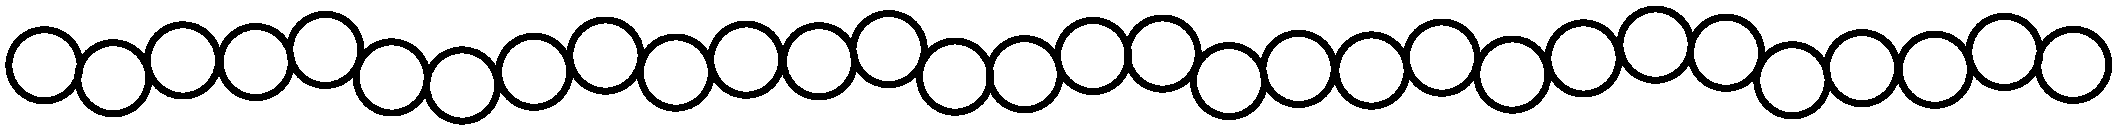
\includegraphics[width=\textwidth]{\figpath/Model1_blank.pdf}}
	
	\question Compare your polymer sequence to those of your group-mates.  What type of sequence (random, alternating, blocky) did this polymerization generally produce?
		
		\begin{solution}[1in]\instructordisplay{
			If done correctly, this simulation will produce completely \emph{random} sequences of monomers.
			
			Example:
			
				\centerline{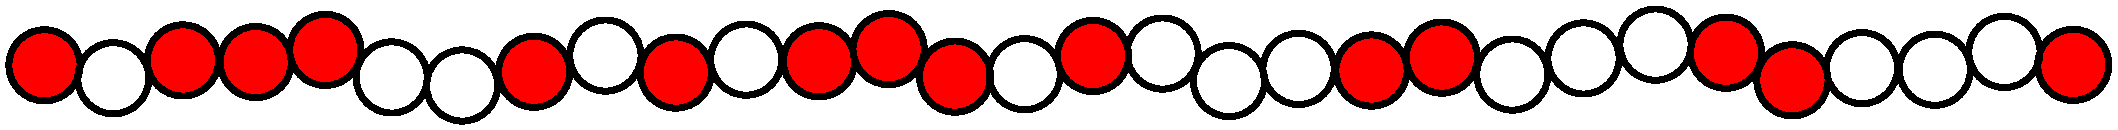
\includegraphics[width=0.5\textwidth]{\figpath/Model1_random.pdf}}
		}\end{solution}
	
	\question \label{\labelbase:ctq:sim-alternating} Repeat the process in Model \ref{\labelbase:mdl:simulation} using the following rules:	\begin{center}
					\renewcommand{\arraystretch}{1.5}
					\begin{tabular}{|c|c|c|}
						\hline
						\textbf{If the last bead was...} &  \textbf{then add an ``A'' bead if} & \textbf{or add a ``B'' bead if}\\\hline
						 an ``A'' bead & Number is $\leq 0.2$ & Number is $> 0.2$ \\\hline
						 a ``B'' bead & Number is $\leq 0.8$ & Number is $> 0.8$ \\\hline
					\end{tabular}
					\end{center}
	
		Then, as before, do the following:
		\begin{enumerate}
			\item Record the sequence of the beads in your chain below.  Shade in the circles corresponding to ``A'' beads, and leave circles corresponding to ``B'' beads blank.
	
		\vspace{6pt}
		\centerline{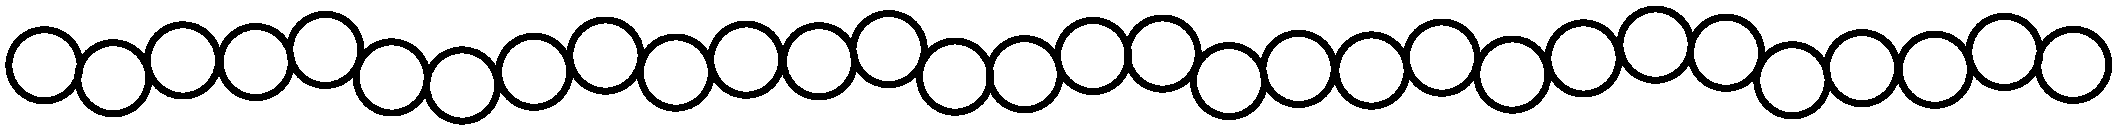
\includegraphics[width=\textwidth]{\figpath/Model1_blank.pdf}}
	
			\item Compare your polymer sequence to those of your group-mates.  What type of sequence (random, alternating, blocky) did this polymerization generally produce?
			
				\begin{solution}[1.25in]\instructordisplay{
					If done correctly, this simulation will produce monomer sequences that tend toward \emph{alternating}.
			
			Example:
			
				\centerline{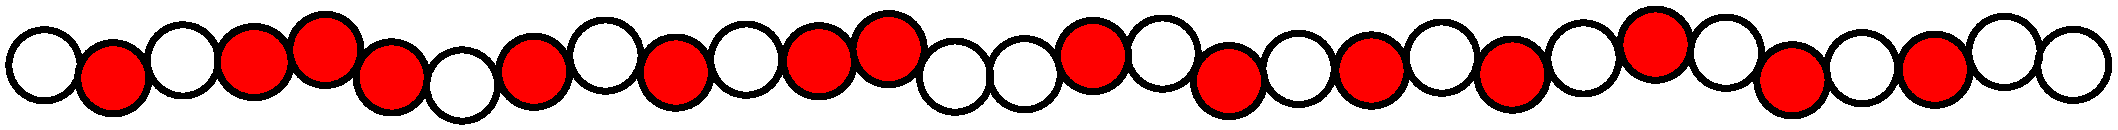
\includegraphics[width=0.5\textwidth]{\figpath/Model1_alternating.pdf}}
				}\end{solution}
				
		\end{enumerate}
		
		\question \label{\labelbase:ctq:sim-blocky} Repeat the process in Model \ref{\labelbase:mdl:simulation} again, this time using the following rules:	\begin{center}
					\renewcommand{\arraystretch}{1.5}
					\begin{tabular}{|c|c|c|}
						\hline
						\textbf{If the last bead was...} &  \textbf{then add an ``A'' bead if} & \textbf{or add a ``B'' bead if}\\\hline
						 an ``A'' bead & Number is $\leq 0.8$ & Number is $> 0.8$ \\\hline
						 a ``B'' bead & Number is $\leq 0.2$ & Number is $> 0.2$ \\\hline
					\end{tabular}
					\end{center}
	
		Then, as before, do the following:
		\begin{enumerate}
			\item Record the sequence of the beads in your chain below.  Shade in the circles corresponding to ``A'' beads, and leave circles corresponding to ``B'' beads blank.
	
		\vspace{6pt}
		\centerline{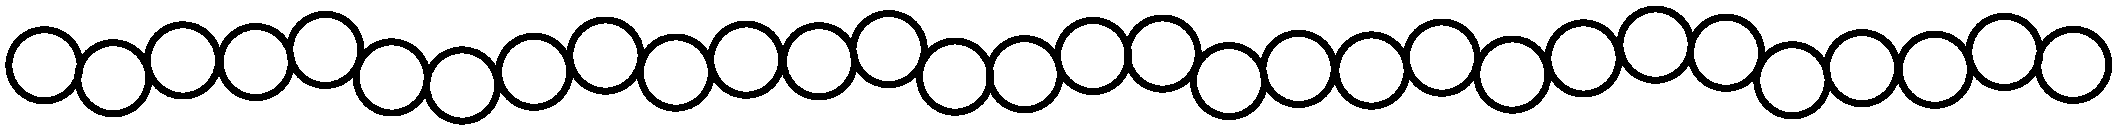
\includegraphics[width=\textwidth]{\figpath/Model1_blank.pdf}}
		
			\item Compare your polymer sequence to those of your group-mates.  What type of sequence (random, alternating, blocky) did this polymerization generally produce?
			
				\begin{solution}[1.5in]\instructordisplay{
					If done correctly, this simulation will produce monomer sequences that tend toward \emph{blocky}.
			
			Example:
			
				\centerline{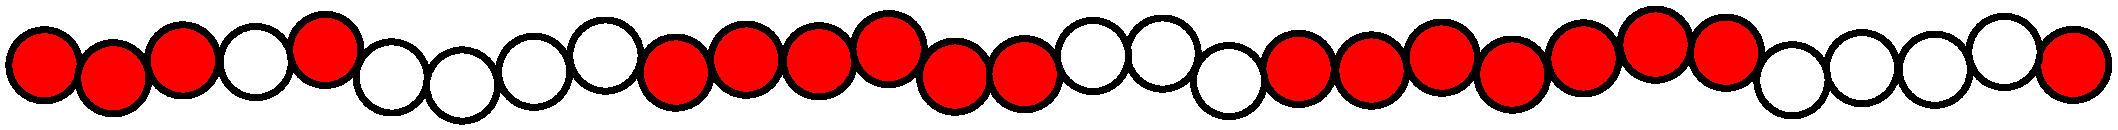
\includegraphics[width=0.5\textwidth]{\figpath/Model1_blocky.pdf}}
				}\end{solution}
		\end{enumerate}
		
	\question \label{\labelbase:ctq:sim-biased} Repeat the process in Model \ref{\labelbase:mdl:simulation} one final time using the following rules:	\begin{center}
					\renewcommand{\arraystretch}{1.5}
					\begin{tabular}{|c|c|c|}
						\hline
						\textbf{If the last bead was...} &  \textbf{then add an ``A'' bead if} & \textbf{or add a ``B'' bead if}\\\hline
						 an ``A'' bead & Number is $\leq 0.2$ & Number is $> 0.2$ \\\hline
						 a ``B'' bead & Number is $\leq 0.2$ & Number is $> 0.2$ \\\hline
					\end{tabular}
					\end{center}
	
		Then, as before, do the following:
		\begin{enumerate}
			\item Record the sequence of the beads in your chain below.  Shade in the circles corresponding to ``A'' beads, and leave circles corresponding to ``B'' beads blank.
	
		\vspace{6pt}
		\centerline{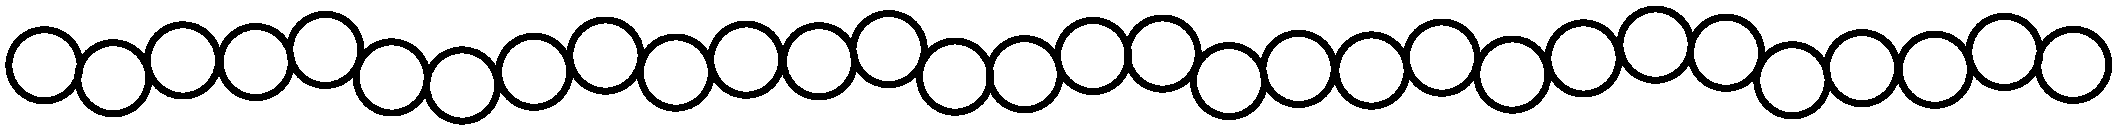
\includegraphics[width=\textwidth]{\figpath/Model1_blank.pdf}}
	
			\item Compare your polymer sequence to those of your group-mates.  What type of sequence (random, alternating, blocky) did this polymerization generally produce?
			
				\begin{solution}[1.25in]\instructordisplay{
					If done correctly, this simulation will produce monomer sequences that are \emph{random}, but \emph{biased} toward incorporation of monomer B.
			
			Example:
			
				\centerline{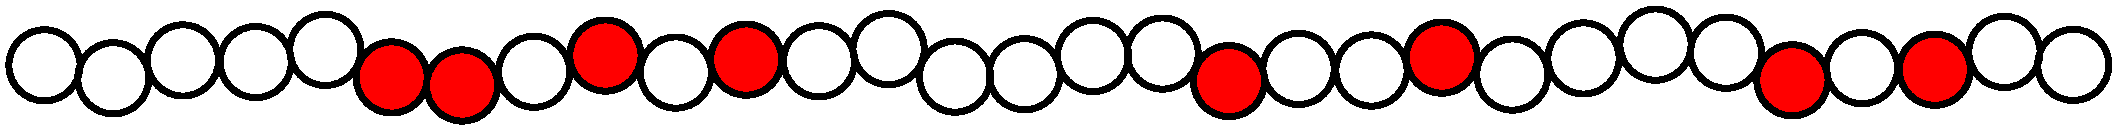
\includegraphics[width=0.5\textwidth]{\figpath/Model1_biased.pdf}}
				}\end{solution}
		\end{enumerate}
		
	\question In which of the simulations did the monomers have the strongest preference for adding monomers of the \emph{same} type?
	
		\begin{solution}[0.85in]\instructordisplay{
			CTQ \ref{\labelbase:ctq:sim-blocky}
		}\end{solution}
	
	\question In which of the simulations did the monomers have the strongest preference for adding monomers of the \emph{other} type?
	
		\begin{solution}[0.85in]\instructordisplay{
			CTQ \ref{\labelbase:ctq:sim-alternating}
		}\end{solution}
	
	\question In which of the simulations did the monomers not ``care'' what type of monomer came before them?
	
		\begin{solution}[0.85in]\instructordisplay{
			CTQs \ref{\labelbase:ctq:sim-random} and  \ref{\labelbase:ctq:sim-biased}
			
			(Note: some students may not put the simulation from CTQ \ref{\labelbase:ctq:sim-biased} into this category, but it does belong here - the probability of adding an ``A'' monomer is the same, no matter what monomer came previously!)
		}\end{solution}
	
	\question In 2-3 complete sentences, describe how the preference of the monomers for adding monomers of the same or different types influences the type of sequence obtained in the copolymerization.
	
		\begin{solution}[2in]
			When the monomers prefer to add to monomers of the same type, we tend to end up with long ``runs'' of the same type of monomer, creating blocky sequences.  On the other hand, when monomers prefer to add to monomers of the opposite type, we tend to end up with alternating sequences.  When there is no preference, the sequence is random, though it may still be biased toward incorporation of one type of monomer or the other.
		\end{solution}
\end{ctqs}

\begin{model}[Kinetics of Copolymerization]
\label{\labelbase:mdl:kinetics}

	In a copolymerization reaction of monomers $M_1$ and $M_2$, there are four possible propagation steps, each with their own rate constant.  These propagation steps are:
	
	\begin{center}
		\renewcommand{\arraystretch}{1.8}
		\begin{tabular}{|c|c|}
			\hline
			\textbf{Reaction} & \textbf{Rate Law} \\\hline
			$-M_1^\bullet + M_1 \xlongrightarrow{k_{11}} -M_1M_1^\bullet$ & $R_{p,11} = k_{11}[-M_1^\bullet][M_1]$ \\\hline
			$-M_1^\bullet + M_2 \xlongrightarrow{k_{12}} -M_1M_2^\bullet$ & $R_{p,12} = k_{12}[-M_1^\bullet][M_2]$ \\\hline
			$-M_2^\bullet + M_1 \xlongrightarrow{k_{21}} -M_2M_1^\bullet$ & $R_{p,21} = k_{21}[-M_2^\bullet][M_1]$ \\\hline
			$-M_2^\bullet + M_2 \xlongrightarrow{k_{22}} -M_2M_2^\bullet$ & $R_{p,22} = k_{22}[-M_2^\bullet][M_2]$ \\\hline
		\end{tabular}
	\end{center}

\end{model}

\begin{ctqs}

	\question Suppose a propagating chain has an $M_1^\bullet$ radical on its active end.  If $R_{p,11}>R_{p,12}$, will the chain be more likely to add an $M_1$ or an $M_2$ monomer next?
	
		\begin{solution}[0.5in]
			$M_1$ (the rate is faster to add an $M_1$ monomer)
		\end{solution}
	
	\question Explain, in 1-2 complete sentences, how the ratio $R_{p,11}/R_{p,12}$ should be related to the relative probability for a chain ending in $M_1^\bullet$ to add another monomer of type $M_1$.
	
		\begin{solution}[1in]
			When $R_{p,11}/R_{p,12} > 1$, it should be more probably to add a monomer of type 1 than a monomer of type 2 because the addition of the type-1 monomer is faster.  When $R_{p,11}/R_{p,12}< 1$, it is more probable to add a monomer of type 2 than a monomer of type 1 because the addition of the type-2 monomer is faster.
		\end{solution}
	
	\question The rates investigated in the previous question depend on the concentrations of the monomers.  If both monomers are present in equal concentration (i.e. $[M_1]=[M_2]$), what is the value of this ratio in terms of the rate constants $k_{11}$ and $k_{12}$?
	
		\begin{solution}[1in]\instructordisplay{
		
			\begin{equation*}
				\frac{R_{p,11}}{R_{p,12}} = \frac{k_{11}[-M_1^\bullet][M_1]}{k_{12}[-M_1^\bullet][M_2]} = \frac{k_{11}[M_1]}{k_{12}[M_2]}
			\end{equation*}
			If $[M_1]=[M_2]$, then this ratio simplifies to $k_{11}/k_{12}$.
		}\end{solution}
	
	\question Explain, in 1-2 complete sentences, why the ratio $k_{11}/k_{12}$ is related to the relative ``preference'' for a chain ending in $M_1^\bullet$ to add another monomer of type $M_1$.
	
		\begin{solution}[1.5in]
			The ratio $k_{11}/k_{12}$ tells us whether the chain is more likely to add a monomer of type 1 or a monomer of type 2 \emph{if} there are equal amounts of each monomer available.  In other words, this tells us what the chain would ``prefer'' to do if there are no restrictions based on one type of monomer being more available than the other.
		\end{solution}
	
\end{ctqs}

\begin{infobox}

	We typically  describe the relative reactivities of monomers 1 and 2 using \emph{reactivity ratios}, $r_1$ and $r_2$, which are defined as
	\begin{align*}
		r_1 = \frac{k_{11}}{k_{12}} && r_2 = \frac{k_{22}}{k_{21}}
	\end{align*}

\end{infobox}

\begin{ctqs}

	\question In Model \ref{\labelbase:mdl:simulation}, the rates of each monomer addition were essentially the probabilities for adding each type of monomer.  Using this information, determine the reactivity ratios for each of the copolymerizations you carried out in Model \ref{\labelbase:mdl:simulation}:
	
		\begin{center}
		\renewcommand{\arraystretch}{2.5}
		\begin{tabular}{|c|c|c|}
			\hline
			\textbf{Simulation} & ~~~~~~$r_1$~~~~~~ & ~~~~~~$r_2$~~~~~~ \\\hline
			\textbf{Model 1/CTQ 1} & \answer{$\frac{0.5}{0.5}=1$} & \answer{$\frac{0.5}{0.5}=1$} \\\hline
			\textbf{CTQ 3} & \answer{$\frac{0.2}{0.8}=0.25$} & \answer{$\frac{0.2}{0.8}=0.25$} \\\hline
			\textbf{CTQ 4} & \answer{$\frac{0.8}{0.2}=4$} & \answer{$\frac{0.8}{0.2}=4$} \\\hline
			\textbf{CTQ 5} & \answer{$\frac{0.2}{0.8}=0.25$} & \answer{$\frac{0.8}{0.2}=4$} \\\hline
		\end{tabular}
		\end{center}

	\question Based on what you learned in Model \ref{\labelbase:mdl:simulation}, what type of sequence (random, alternating, blocky, etc.) do you expect when...
	
		\begin{enumerate}
			\item $r_1 = 1$ and $r_2$ = 1?
			
				\begin{solution}[0.5in]
					random, unbiased
				\end{solution}
			
			\item $r_1 = \frac{1}{r_2} \neq 1$?
			
				\begin{solution}[0.5in]
					random but biased toward one type of monomer
				\end{solution}
			
			\item $r_1 < 1$ and $r_2 < 1$?
			
				\begin{solution}[0.5in]
					alternating (1'2 prefer to add 2's and 2's prefer to add 1's)
				\end{solution}
			
			\item $r_1 > 1$ and $r_2 > 1$?
			
				\begin{solution}[0.5in]
					blocky (1's prefer to add 1's and 2's prefer to add 2's)
				\end{solution}
		\end{enumerate}

\end{ctqs}

\vspace{0.5in}
\begin{model}[Feed Ratios]
	\label{\labelbase:mdl:feedratios}
	
	Often, the most important thing for us to know is how the composition of the polymer being formed is related to the composition of the monomer mixture.  We quantify this relationship using two values:
	\begin{itemize}
		\item the \emph{feed ratio}, $f_1$, is the fraction of the \emph{unreacted} monomers that are type $M_1$
		\item the \emph{polymer composition}, $F_1$, is the fraction of  the monomers \emph{in the polymer} that are type $M_1$
	\end{itemize}
	
	Working through the kinetics, we find that the polymer composition is related to the feed ratio by
	\begin{equation*}
		F_1 = \frac{r_1f_1^2 + f_1f_2}{r_1f_1^2+2f_1f_2 + r_2f_2^2}
	\end{equation*}
	where $f_2 = 1-f_1$.

\end{model}

\clearpage
\begin{ctqs}
	\question \label{\labelbase:ctq:f1F1plot} A plot of $F_1$ vs. $f_1$ is shown below for $r_1 = 4$, $r_2=0.25$: 
	
		\vspace{3pt}
		\centerline{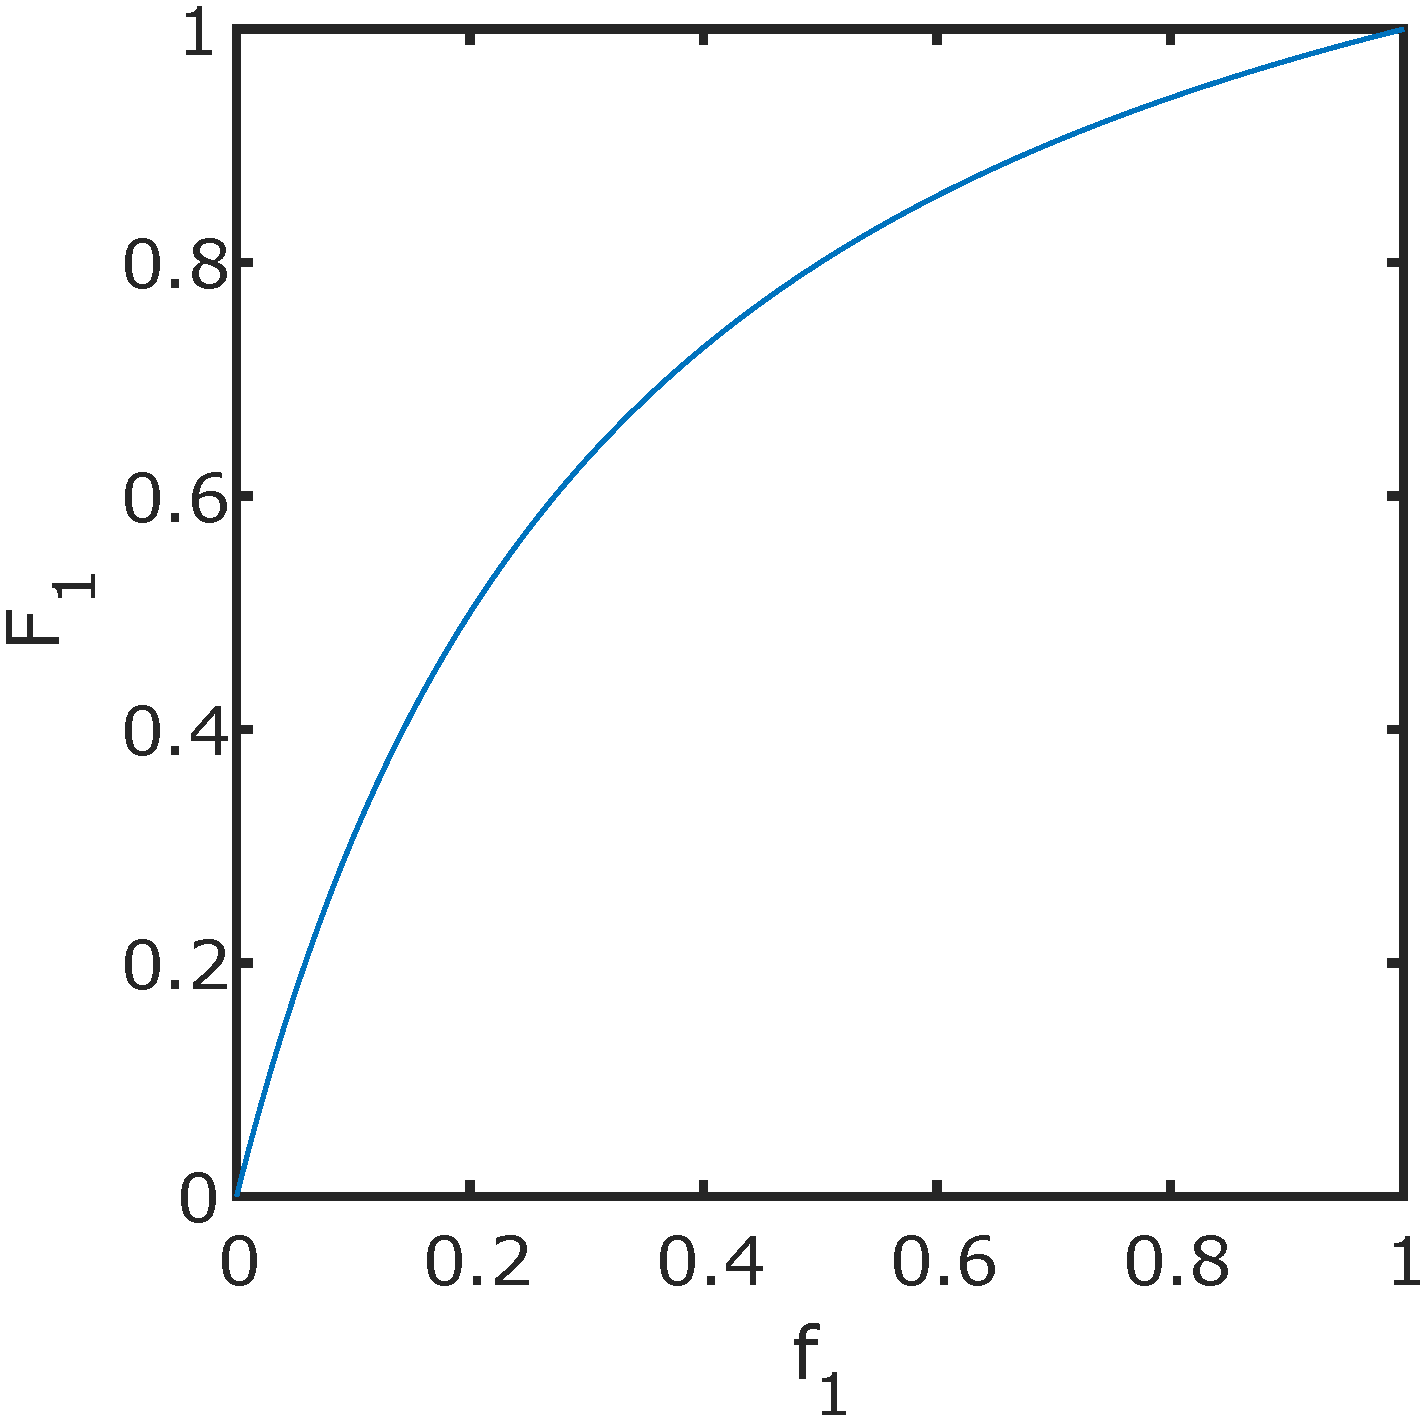
\includegraphics[width=0.35\textwidth]{\figpath/Model3_r1-4_r2-0,25.pdf}}
	
		Qualitatively, why should $r_1 = 4$, $r_2=0.25$ generate this shape of plot?  Briefly explain your reasoning in 1-2 complete sentences.
				
		\begin{solution}[1.5in]\instructordisplay{
			As discussed in Model \ref{\labelbase:mdl:kinetics}, $r_1=4$ and $r_2=0.25$ indicate that chains ending in either monomer type will always prefer to add a new monomer of type 1.  As a consequence, the polymer composition will always be enriched in monomer 1 relative to the feed, so $F_1$ will always be greater than $f_1$.
		}\end{solution}
		
	\question Consider a reaction mixture that contains exactly 50\% $M_1$ monomers and 50\% $M_2$ monomers.
	
		\begin{enumerate}
			\item What is the value of $f_1$ for this reaction mixture?
			
				\begin{solution}[0.5in]
					exactly 50\% of the monomers are type 1, so $f_1=0.5$
				\end{solution}
			
			\item Assuming the reactivity ratios are the same as in CTQ \ref{\labelbase:ctq:f1F1plot}, what fraction of the monomers \emph{in the polymer} will be type $M_1$?
			
				\begin{solution}[0.5in]
					0.8 (students can either calculate this using the equation in the Model, or estimate off the plot)
				\end{solution}
			
			\item As the reaction goes, what will happen to the concentration of monomer $M_1$ left in solution?
				
				\begin{solution}[1in]
					Because $M_1$ is being preferentially incorporated into the polymer, the concentration of $M_1$ left in solution will decrease (more so than the concentration of $M_2$ will)
				\end{solution}
			\item Predict how the values of $f_1$ and $F_1$ are likely to change over time in this reaction.
				
				\begin{solution}[1in]\instructordisplay{
					As the amount of $M_1$ decreases, the value of $f_1$ will decrease.  The value of $F_1$ will then also decrease over time - the composition of the polymer will gradually shift to contain fewer $M_1$ (and more $M_2$) monomers.
					
					Exercise \ref{\labelbase:exc:compshift} asks students to think through how this composition drift will affect the composition and/or sequence of the resulting polymers.
				}\end{solution}
			
			
		\end{enumerate}
		
	\question \label{\labelbase:ctq:FinemanRoss} With a little algebra, the equation from Model \ref{\labelbase:mdl:feedratios} can be rewritten
		\begin{equation*}
			\frac{f_1(1-2F_1)}{F_1(1-f_1)} = r_1\left(\frac{f_1^2(F_1-1)}{F_1(1-f_1)^2}\right)+r_2
		\end{equation*}
		
		\begin{enumerate}
			\item Rewrite this equation using the substitutions $y=\frac{f_1(1-2F_1)}{F_1(1-f_1)}$ and $x=\left(\frac{f_1^2(F_1-1)}{F_1(1-f_1)^2}\right)$.  What type of equation results?
			
				\begin{solution}[1in]\instructordisplay{
					The resulting equation is
					\begin{equation*}
						y = r_1 x + r_2
					\end{equation*}
					This is a linear equation ($y=mx+b$), where the slope $m$ is $r_1$ and the intercept $b$ is $r_2$.
				}\end{solution}
			
			\item Using your answer to the previous question, propose a method that you could use to determine the reactivity ratios for a pair of monomers if given values of $F_1$ corresponding to a range of different $f_1$ values.
			
				\begin{solution}[2in]\instructordisplay{
					A simple way to find $r_1$ and $r_2$ would be to plot $\frac{f_1(1-2F_1)}{F_1(1-f_1)}$ vs  $\left(\frac{f_1^2(F_1-1)}{F_1(1-f_1)^2}\right)$ and fit the data to a line.  The slope of the line would be $r_1$ and the intercept would be $r_2$.
				}\end{solution}
		\end{enumerate}
\end{ctqs}


\begin{exercises}

	\exercise Make plots analogous to the plot in CTQ \ref{\labelbase:ctq:f1F1plot} for each of the following pairs of reactivity ratios.  For each plot, explain why it has the shape that it does, and predict how the composition of the polymer would change with time for a polymerization that starts at $f_1=0.5$.
	
		\begin{enumerate}
			\item $r_1=1$, $r_2=1$:
	
				\begin{solution}\instructordisplay{
					\centerline{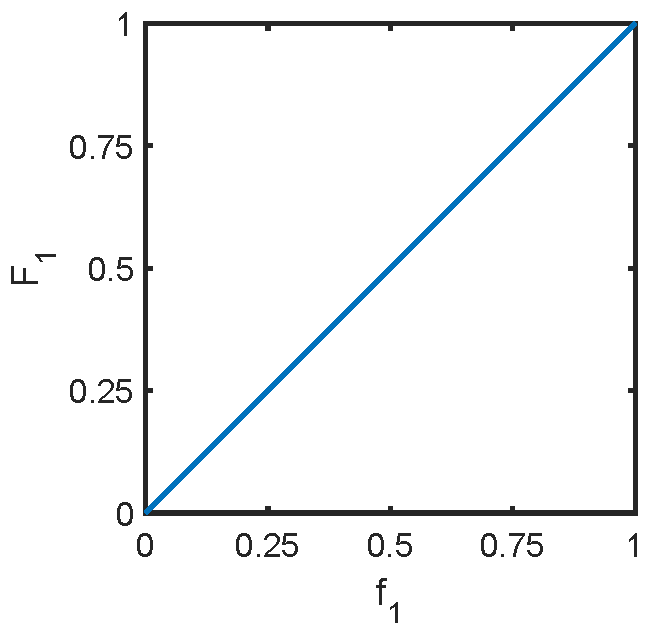
\includegraphics[width=0.35\textwidth]{\figpath/Exercises_1a.pdf}}
				
					Because the reactivity ratios are both 1, neither monomer has a preference regarding which type of monomer adds next, so the composition of the polymer ($F_1$) should always just directly amtch the composition of the monomer mixture ($f_1$), yielding a straight line.
					
					Because $F_1=f_1$, the composition of the feed ratio will not change with time, and neither will the composition of the polymer.
		
				}\end{solution}		

			\item $r_1=0.1$, $r_2=10$:
			
				\begin{solution}\instructordisplay{
	
					\centerline{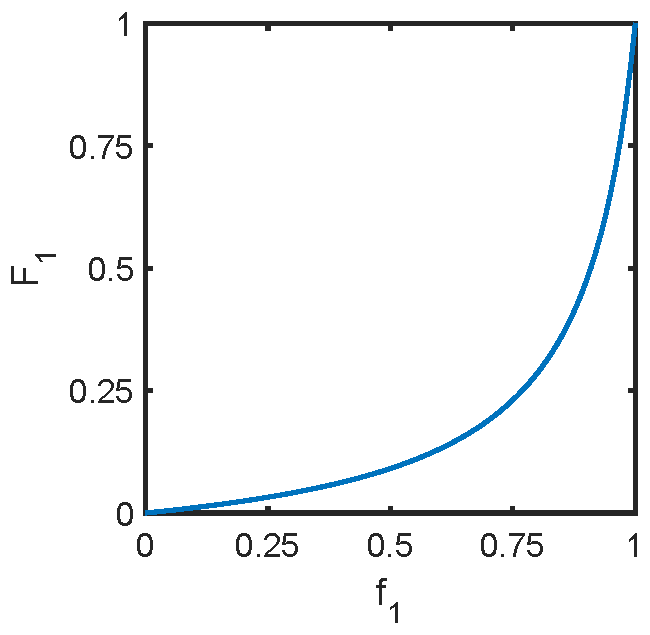
\includegraphics[width=0.35\textwidth]{\figpath/Exercises_1b.pdf}}
				
					In this case, both monomers have a strong preference to add monomer 2 as the next monomer instead of monomer 1.  As a result, the polymer composition will always be enriched in monomer 2 (or depleted in monomer 1) relative to the composition of the monomer mixture; $F_1$ will always be less than $f_1$.
					
					Because $F_1<f_1$, the monomer feed (and thus the polymer composition) will become progressively enriched in monomer !.
					
				}\end{solution}
				
				
			\item $r_1=0.33$, $r_2=0.67$:
	
				\begin{solution}\instructordisplay{
					\centerline{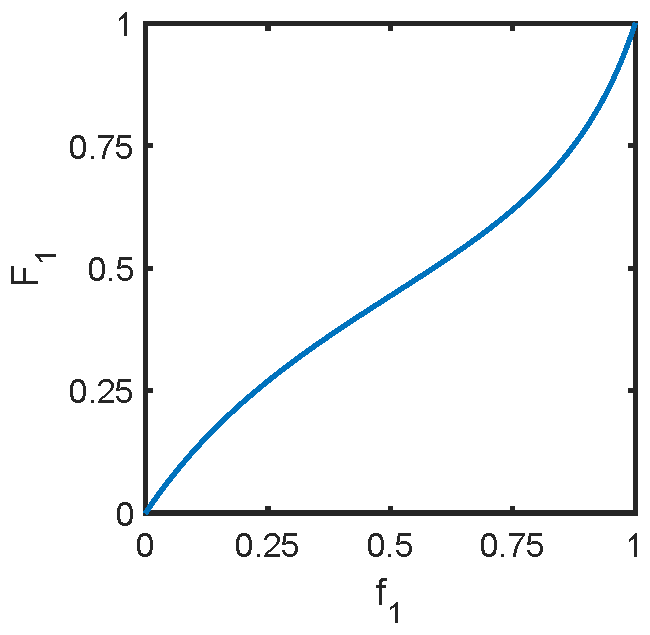
\includegraphics[width=0.35\textwidth]{\figpath/Exercises_1c.pdf}}
					
					In this case, both monomers have a slight preference for adding the other monomer, although it is not a particularly strong preference (the reactivity ratios are only slightly lower than one).  When there is a large excess of monomer 1 in the reaction mixture ($f_1$ is large), more chains will end in monomer 1 and will prefer adding monomer 2, meaning that the polymer composition will have less of monomer 1 than is in the reaction mixture (i.e. when $f_1$ is large, $F_1<f_1$).  On the other hand, when there is an excess of monomer 2 ($f_1$ is small), more chains will end in monomer 2 and will prefer adding monomer 1, meaning that the polymer composition will have more of monomer 1 than is in the reaction mixture (i.e. when $f_1$ is small, $F_1 > f_1$).  This gives the characteristic S-shaped curve seen in this graph.
					
					For a monomer mixture prepared at $f_1=0.5$, the initial polymer composition will be approximately $F_1=0.44$.  As a result, the monomer feed (and thus the polymer composition) will become progressively enriched in monomer 1 as the reaction progresses.
			}\end{solution}
		\end{enumerate}
	
	\exercise In CTQ \ref{\labelbase:ctq:f1F1plot}, you predicted how the values of $f_1$ and $F_1$ are likely to change over the course of a reaction.  For the reactivity ratios described in this question, do the following: \label{\labelbase:exc:compshift}
	
		\begin{enumerate}
			\item Briefly describe the characteristics of the polymer that you expect to obtain if the polymerization is carried out under free radical conditions.
			
				\emph{Hint: in a free radical polymerization, the lifetime of any individual radical is very short relative to the overall reaction time!}
			
				\begin{solution}\instructordisplay{
					The resulting polymer would be compositionally heterogeneous, with polymer chains formed early in the reaction having more of monomer $M_1$ and polymer chains formed later in the reaction being (relatively) enriched in $M_2$.
					
					The individual chains would not have a significant gradient structure, since the radical lifetime is short and each propagating radical essentially sees an instantaneously fixed value of $f_1$ over its lifetime.
				}\end{solution}
				
			\item Briefly describe the characteristics of the polymer that you expect to obtain if this polymerization were carried out using RAFT or ATRP.
			
				\begin{solution}\instructordisplay{
					In a controlled radical polymerization, the chains grow slowly enough that they will see the composition drift in the mixture.  The resulting chains will thus have a gradient structure that is enriched in monomer $M_1$ on the initiator end and in monomer $M_2$ on the terminating end.
				}\end{solution}
				
		\end{enumerate}
	
	%\exercise Quantify probabilities from rate data in model 2?
	
\end{exercises}


%\begin{problems}
%
%	\problem First exercise
%	\problem Second exercise
%	
%\end{problems}


	
\end{activity}